%------------------------------
% CHAPTER: Algorithm Specification
%------------------------------
\chapter{Algorithm Specification}
\label{ch:AlgorithmSpec}
Our authenticated encryption algorithm is based on the simplified duplex construction.
Padding and domain separation are assumed to be done at some higher level in the overall system if needed.
For this reason, it is sufficient to specify only the duplex parameters and the sponge function $f$.

For Known Answer Tests (KATs) corresponding to this specification, see Appendix~\ref{appx:KATs}.

\section{Duplex Parameters}
We allow two key sizes: $128$ bits and $256$ bits.
These are the NIST recommended symmetric key sizes as of 2011 \cite{NIST2011_KeySizes}.
Our construction uses a $512$-bit internal state, so we have $b = 512$.
The rate $r$ is $128$ bits for both key lengths, which means that the capacity $c$ is $384$.
Keeping the rate at a constant $128$ bits for both instantiations means that switching between key lengths is a trivial task.

The capacity $c = 384$ provides sufficient security against generic attacks for both $128$- and $256$-bit keys.
As explained in Chapter~\ref{ch:SpongeAndDuplex}, we know from \cite{Jovanovic2014_Beyond} that the generic security level is
\begin{equation*}
\mathrm{min}(2^{(r+c)/2}, 2^c, 2^{|K|}).
\end{equation*}
For a $128$-bit key, the security level is $2^{128}$.
For a $256$-bit key, the security level is $2^{256}$. 

\section{Permutation $f$}
Our underlying sponge function $f$ is a permutation, so it has the advantage of being fully entropy-preserving.
Since it is bijective, $f^{-1}$ exists by definition.
We specify both $f$ and $f^{-1}$ here.
While $f^{-1}$ is never used in practice, it may be useful for cryptanalysis and verification purposes.

\begin{figure}[p,height=.8\textheight]
\centering
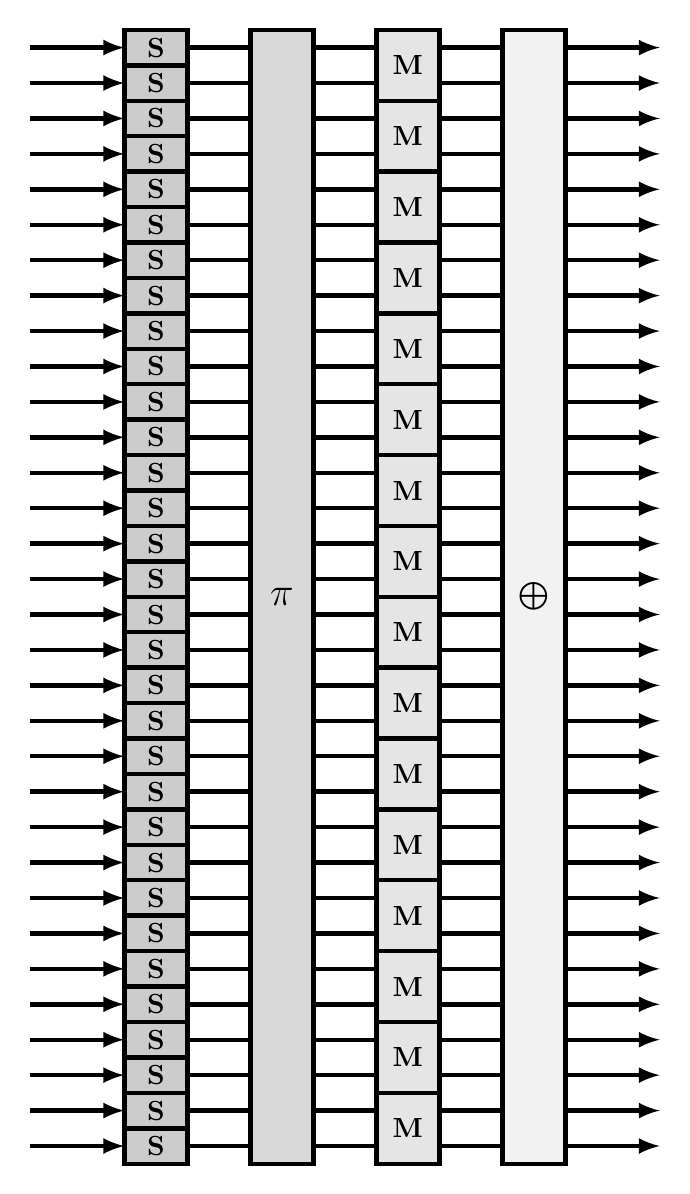
\begin{tikzpicture}[xscale=.8,yscale=0.45,>=latex,ultra thick]
% Reference grid (temporary)
%\draw[help lines] (0,0) grid (16,32);

% TODO label bits / words

% Entry arrows
\foreach \i in {32,...,1} {
  \draw[->] (-1.5,\i-0.5) -- (0,\i-0.5);
}

% Wires
\foreach \j in {1,3,5} {
  \foreach \i in {32,...,1} {
    \draw (\j,\i-0.5) -- (\j+1,\i-0.5);
  }
}

% S-boxes
\foreach \i in {32,...,1} {
  \draw[fill=gray!40] (0,\i) rectangle (1,\i-1) node[midway] {$\mathbf{S}$} ;
}

% P-boxes
\draw[fill=gray!30] (2,0) rectangle (3,32) node[midway] {\Large$\mathbf{\pi}$};

% Mixers
\foreach \i in {32,30,...,2} {
  \draw[fill=gray!20] (4,\i) rectangle (5,\i-2) node[midway] {$\mathbf{M}$};
}

% Round key box
\draw[fill=gray!10] (6,0) rectangle (7,32) node[midway] {$\bigoplus$};

% Exit arrows
\foreach \i in {32,...,1} {
  \draw[->] (7,\i-0.5) -- (8.5,\i-0.5);
}

\end{tikzpicture}


\caption{A single round of the sponge permutation $f$. Each line represents a $16$-bit word.}
\label{fig:Round}
\end{figure}

\begin{figure}[p,height=.8\textheight]
\centering
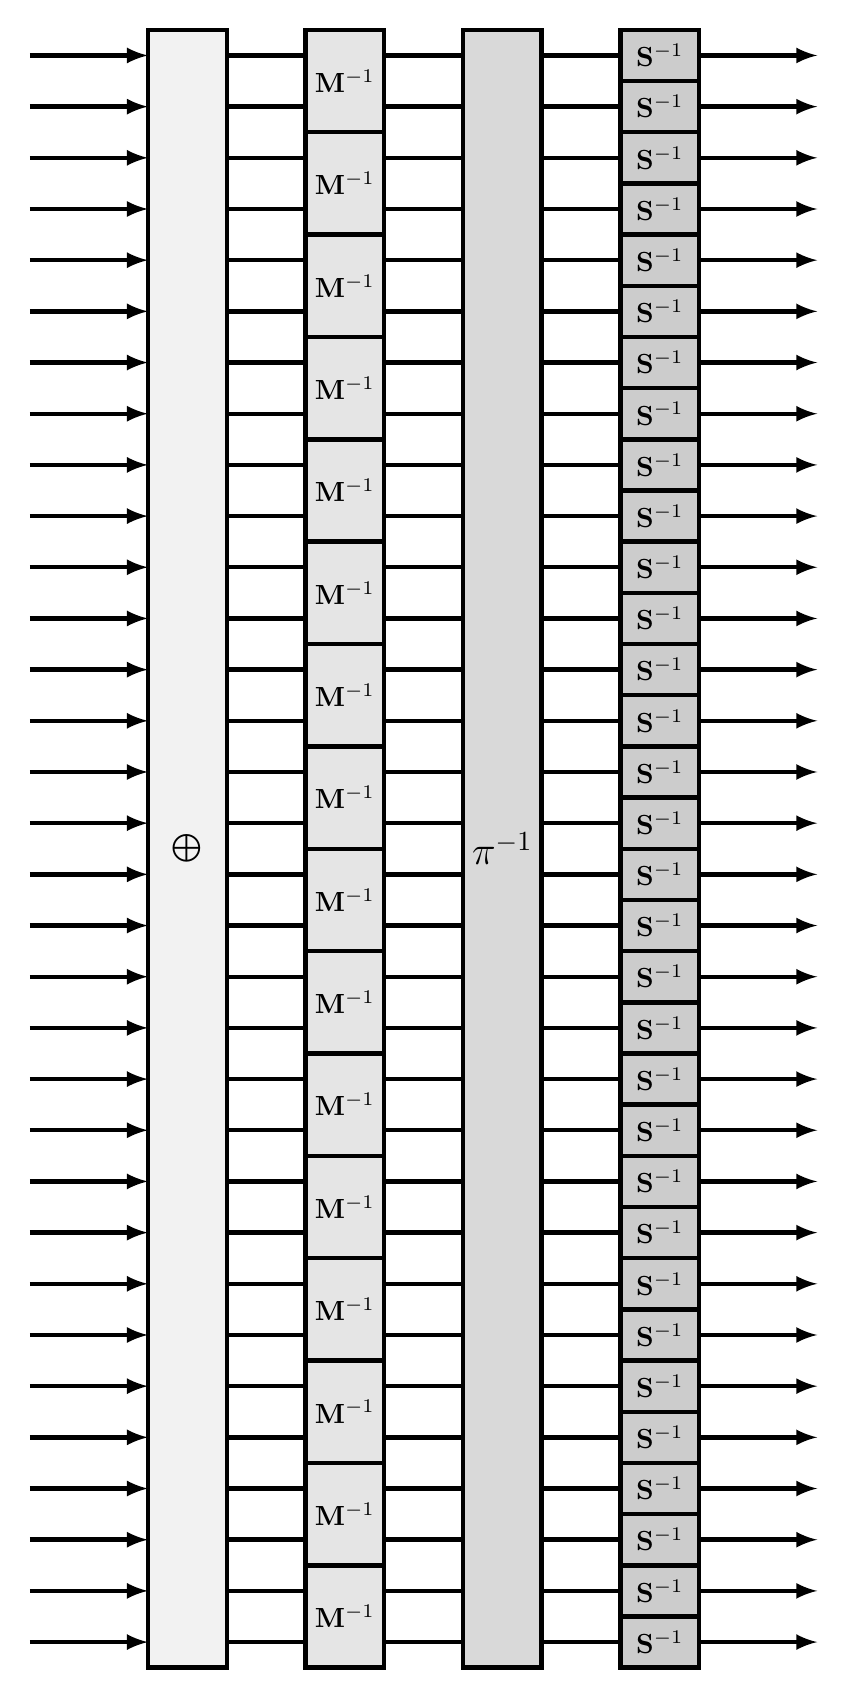
\begin{tikzpicture}[xscale=1,yscale=0.65,>=latex,ultra thick]
% Reference grid (temporary)
%\draw[help lines] (0,0) grid (16,32);

% Entry arrows
\foreach \i in {32,...,1} {
  \draw[->] (-1.5,\i-0.5) -- (0,\i-0.5);
}

% Wires
\foreach \j in {1,3,5} {
  \foreach \i in {32,...,1} {
    \draw (\j,\i-0.5) -- (\j+1,\i-0.5);
  }
}

% Round key box
\draw[fill=gray!10] (0,0) rectangle (1,32) node[midway] {$\bigoplus$};

% Mixers
\foreach \i in {32,30,...,2} {
  \draw[fill=gray!20] (2,\i) rectangle (3,\i-2) node[midway] {$\mathbf{M}^{-1}$};
}

% P-boxes
\draw[fill=gray!30] (4,0) rectangle (5,32) node[midway] {\Large$\mathbf{\pi}^{-1}$};

% S-boxes
\foreach \i in {32,...,1} {
  \draw[fill=gray!40] (6,\i) rectangle (7,\i-1) node[midway] {$\mathbf{S}^{-1}$} ;
}


% Exit arrows
\foreach \i in {32,...,1} {
  \draw[->] (7,\i-0.5) -- (8.5,\i-0.5);
}

\end{tikzpicture}


\caption{An inverse round of the permutation $f$. Each line represents a $16$-bit word.}
\label{fig:RoundInverse}
\end{figure}

The permutation consists of a number of rounds.
Figure~\ref{fig:Round} shows a diagram of a single round of the forward permutation.
Figure~\ref{fig:RoundInverse} shows a single inverse round.
Each round can be represented as the composition of several subfunctions or \emph{steps}: a substitution, a bitwise permutation, a mixing layer, and the addition of a round constant.
These are represented respectively as $\mathbf{S}$, $\mathbf{\pi}$, $\mathbf{M}$, and $\oplus$ in the diagrams.

\subsection{Substitution Step}
The substitution step is a bricklayer permutation that uses $32$ identical, bijective $16 \times 16$ S-boxes.
This step is the main source of confusion within the permutation.
Furthermore, it is the only nonlinear step, as is typical with most substitution-based symmetric key algorithms \cite{Stinson2006_CTAP}.

To the best of our knowledge this is the first cryptosytem to use such large S-boxes.
We believe that, at the time of writing, the largest S-boxes used in the literature are the $8 \times 8$ bijective S-boxes used by the Advanced Encryption Standard (AES) \cite{Daemen2002_DesignOfRijndael}\cite{NIST2001_FIPS-197}.

Our S-box is an AES-inspired design taken directly from Wood's thesis on the subject \cite{Wood2013_SboxThesis}.
The primary reason for using this particular class of $16$-bit S-boxes is that they are efficiently implementable in hardware.
Rather than being based on a random mapping, they are based on multiplicative inversion in a finite field followed by an affine transformation.
This allows us to implement an actual circuit which performs the operations rather than use the corresponding (and prohibitively large) look-up table.

Specifically, we use the reference C implementation provided in Appendix C of the aforementioned thesis.
This S-box is based on multiplicative inversion in $\gfsixteen / \left\langle p(x) \right\rangle$ where 
\begin{equation*}
p(x) = x^{16} + x^5 + x^3 + x + 1.
\end{equation*}
We represent an input to the S-box (and inverse S-box) as a $16$-bit column vector 
\begin{equation*}
x = 
\begin{pmatrix}
x_{15} & x_{14} & \ldots & x_1 & x_0
\end{pmatrix}^\mathrm{T},
\end{equation*}
where $x_{15}$ is the MSB.
Using this notation, the forward S-box function is given as
\begin{equation*}
\renewcommand{\arraystretch}{0.7} % Make it square
\mathbf{S}(x) = 
\begin{pmatrix}
0 & 0 & 1 & 0 & 0 & 0 & 0 & 1 & 0 & 0 & 1 & 1 & 1 & 1 & 1 & 0 \\
1 & 1 & 0 & 0 & 0 & 0 & 0 & 1 & 0 & 1 & 1 & 0 & 1 & 0 & 1 & 0 \\
1 & 1 & 0 & 0 & 1 & 0 & 1 & 1 & 0 & 1 & 0 & 1 & 0 & 0 & 1 & 1 \\
1 & 1 & 1 & 0 & 0 & 0 & 1 & 0 & 0 & 1 & 1 & 0 & 0 & 0 & 0 & 0 \\

1 & 1 & 0 & 0 & 0 & 1 & 1 & 0 & 0 & 1 & 1 & 1 & 1 & 0 & 1 & 1 \\
0 & 1 & 0 & 0 & 0 & 0 & 1 & 1 & 0 & 1 & 1 & 1 & 1 & 1 & 0 & 1 \\
0 & 0 & 1 & 0 & 1 & 0 & 1 & 0 & 1 & 1 & 0 & 0 & 1 & 1 & 0 & 0 \\
1 & 0 & 1 & 1 & 1 & 0 & 1 & 1 & 0 & 0 & 0 & 1 & 0 & 1 & 1 & 1 \\

0 & 1 & 0 & 0 & 0 & 0 & 0 & 0 & 1 & 0 & 0 & 1 & 1 & 1 & 0 & 1 \\
1 & 0 & 1 & 1 & 0 & 0 & 0 & 1 & 0 & 0 & 1 & 0 & 1 & 0 & 0 & 0 \\
1 & 0 & 1 & 0 & 0 & 1 & 1 & 1 & 0 & 0 & 1 & 1 & 0 & 1 & 0 & 0 \\
1 & 0 & 1 & 1 & 1 & 0 & 1 & 1 & 1 & 1 & 0 & 1 & 1 & 0 & 0 & 1 \\

1 & 0 & 1 & 0 & 0 & 1 & 0 & 1 & 1 & 0 & 0 & 1 & 0 & 0 & 0 & 1 \\
0 & 1 & 0 & 0 & 0 & 1 & 1 & 1 & 1 & 0 & 0 & 0 & 0 & 0 & 0 & 1 \\
1 & 0 & 0 & 0 & 1 & 1 & 0 & 1 & 0 & 1 & 1 & 1 & 1 & 0 & 0 & 0 \\
1 & 1 & 0 & 1 & 0 & 1 & 1 & 0 & 1 & 0 & 0 & 1 & 1 & 0 & 0 & 0 \\
\end{pmatrix}
\begin{pmatrix}
x_{15} \\
x_{14} \\
x_{13} \\
x_{12} \\
x_{11} \\
x_{10} \\
x_{9} \\
x_{8} \\
x_{7} \\
x_{6} \\
x_{5} \\
x_{4} \\
x_{3} \\
x_{2} \\
x_{1} \\
x_{0} \\
\end{pmatrix}
^{-1}
\oplus
\begin{pmatrix}
0 \\
1 \\
0 \\
0 \\
0 \\
1 \\
0 \\
1 \\
1 \\
0 \\
1 \\
1 \\
0 \\
1 \\
1 \\
1 \\
\end{pmatrix}
\end{equation*}
and the inverse is
\begin{equation*}
\renewcommand{\arraystretch}{0.7} % Make it square
\mathbf{S}^{-1}(x) = 
\left[
\begin{pmatrix}
0 & 1 & 0 & 1 & 0 & 1 & 1 & 1 & 0 & 0 & 1 & 0 & 0 & 0 & 0 & 1 \\
1 & 1 & 0 & 1 & 0 & 0 & 1 & 0 & 1 & 0 & 1 & 1 & 1 & 1 & 0 & 1 \\
1 & 0 & 1 & 1 & 1 & 1 & 0 & 1 & 0 & 1 & 1 & 0 & 0 & 0 & 0 & 0 \\
0 & 0 & 1 & 0 & 1 & 1 & 1 & 0 & 1 & 0 & 1 & 1 & 1 & 0 & 1 & 0 \\

1 & 1 & 1 & 1 & 1 & 0 & 0 & 0 & 1 & 0 & 0 & 0 & 0 & 1 & 0 & 0 \\
0 & 0 & 0 & 1 & 0 & 1 & 0 & 0 & 0 & 0 & 1 & 1 & 1 & 1 & 1 & 1 \\
1 & 0 & 1 & 0 & 0 & 0 & 0 & 0 & 0 & 1 & 1 & 0 & 1 & 0 & 1 & 1 \\
0 & 0 & 1 & 0 & 1 & 1 & 1 & 0 & 0 & 1 & 0 & 1 & 1 & 1 & 1 & 0 \\

0 & 0 & 0 & 0 & 0 & 0 & 1 & 0 & 0 & 0 & 1 & 0 & 0 & 0 & 1 & 0 \\
1 & 1 & 1 & 0 & 0 & 1 & 1 & 1 & 1 & 0 & 1 & 1 & 1 & 0 & 0 & 0 \\
0 & 1 & 1 & 0 & 1 & 1 & 1 & 1 & 0 & 0 & 1 & 0 & 1 & 1 & 1 & 1 \\
1 & 0 & 0 & 1 & 1 & 0 & 0 & 0 & 1 & 0 & 0 & 1 & 1 & 0 & 1 & 1 \\

1 & 0 & 0 & 0 & 0 & 1 & 0 & 1 & 1 & 1 & 0 & 0 & 1 & 0 & 1 & 0 \\
1 & 0 & 0 & 0 & 0 & 1 & 1 & 1 & 1 & 1 & 0 & 1 & 1 & 1 & 1 & 1 \\
1 & 1 & 1 & 0 & 0 & 1 & 1 & 0 & 1 & 0 & 0 & 1 & 1 & 1 & 1 & 1 \\
0 & 1 & 0 & 0 & 1 & 0 & 1 & 0 & 1 & 0 & 0 & 1 & 0 & 0 & 0 & 1 \\
\end{pmatrix}
\begin{pmatrix}
x_{15} \\
x_{14} \oplus 1 \\
x_{13} \\
x_{12} \\
x_{11} \\
x_{10} \oplus 1 \\
x_{9} \\
x_{8} \oplus 1 \\
x_{7} \oplus 1 \\
x_{6} \\
x_{5} \oplus 1 \\
x_{4} \oplus 1 \\
x_{3} \\
x_{2} \oplus 1 \\
x_{1} \oplus 1 \\
x_{0} \oplus 1 \\
\end{pmatrix}
\right]^{-1}.
\end{equation*}

A hardware implementation for this particular S-box requires just $1238$ XOR gates and $144$ AND gates.
However, No concrete implementation (e.g.\ in VHDL) is provided; this is an area for future work.

\subsection{Bitwise Permutation Step}
Bitwise permutations are easily implementable in hardware via a simple rerouting of wires.
Compared to a permutation on the words of the state, a bitwise permutation intuitively provides much better diffusion.
The bitwise permutation step is the main source of long-range (i.e.\ across the entire state) diffusion in the algorithm.

The bitwise permutation also helps maximize the minimum number of active S-boxes by being subject to certain constraints.
We use a permutation that satisfies the following properties:
\begin{enumerate}
\item All outputs of a given S-box go to $16$ different mixers
\item The permutation is a \emph{derangement}; it has no fixed points
\item High order; it does not repeat within the number of rounds
\item No low order bits; the order of any bit equals the order of the overall permutation
\item Easily definable by some function
\end{enumerate}
There is obviously no cryptographic significance to how ``easy'' it is to express a bitwise permutation.
This is merely to cut down on the search space and to avoid having to provide a table with $512$ entries to express the permutation.

We denote the bitwise permutation function
\begin{equation*}
\pi \from \mathbb{Z}_{512} \to \mathbb{Z}_{512},
\end{equation*}
where it operates on the \emph{index} of a given bit, $x \in \mathbb{Z}_{512}$. 

To understand our specific choice of $\pi$, it is useful to consider a poor choice first.
For this we can turn our attention to the lightweight block cipher PRESENT which operates on a $64$-bit state over $31$ rounds.
PRESENT uses the bitwise permutation
\begin{equation*}
\pi_P \from \mathbb{Z}_{63} \to \mathbb{Z}_{63}
\end{equation*}
given by the linear function
\begin{equation*}
\pi_P(x) = 16x \bmod{63}.
\end{equation*}
Since it operates in $Z_{63}$, an augmented mapping $\pi_P(63) = 63$ is required for the last bit \cite{Bogdanov2007_PRESENT}.

The particular structure of $\pi_P$ led to an attack on PRESENT in 2009 \cite{Nakahara2009_PRESENT_Cryptanalysis}.
The attack leverages the following undesirable properties of $\pi_P$:
\begin{enumerate}
\item There are four fixed points: $x = 0, 21, 41, 63$
\item The order is only three: $\pi_P^3(x) = \pi_P(x)$
\end{enumerate}
The combination of these properties results in a decrease in the lower bound on the number of active S-boxes across four rounds since it is possible to construct a trail that branches back into itself after $\pi_P$ is iterated only three times.
See Figure~\ref{fig:PRESENT_Trail} for a diagram that illustrates this trail.

A simple way to avoid fixed points is to use an affine function rather than a linear function.
An affine function over $\mathbb{Z}_{512}$ is of the form
\begin{equation*}
\pi(x) = \alpha x + \beta \bmod{512}.
\end{equation*}
For $\pi$ to be bijective, we require $\gcd(\alpha, 512) = 1$.
Since the prime factorization of $512$ is simply $2^9$, it is equivalent to say that $\alpha$ must be odd \cite{Stinson2006_CTAP}.

A low order bit is defined as a bit that has order less than the order of the overall bitwise permutation.
It is cumbersome to mathematically characterize all permutations that satisfy the property that no bits have low order. Instead, we wrote a script (see Appendix~\ref{appx:SourceCodeListings}) to search for such permutations.
The script also identifies if a given permutation satisfies all other properties that we require.
We found $384$ permutations defined by affine functions over $Z_{512}$ that satisfy all properties. A complete listing is provided in Table~\ref{tab:BitwisePermutations}.

We chose the following permutation to use for our algorithm since it is the first function to satisfy all properties:
\begin{equation*}
\pi(x) = 31x + 15 \bmod{512}
\end{equation*}
This particular bitwise permutation has order $32$ and its inverse is given by
\begin{equation*}
\pi^{-1}(x) = 479(x-15) \bmod{512}
\end{equation*}
since $31^{-1} \equiv 479$ in $\mathbb{Z}_{512}$.

\subsection{Mix Step}
The purpose of the mix step is to provide local diffusion (i.e.\ across two words) and increase the linear and differential branch numbers of a round from two to three.
See Chapter~\ref{ch:Cryptanalysis} for more detail on branch numbers.
We use a mixer based on multiplication by a $2 \times 2$ matrix in \gfsixteen modulo the irreducible polynomial
\begin{equation*}
p(x) = x^{16} + x^5 + x^3 + x^2 + 1.
\end{equation*}
The mixer takes two words $A$ and $B$ as input and produces outputs $A'$ and $B'$ as follows:
\begin{equation*}
\begin{pmatrix}
A' \\ B'
\end{pmatrix}
=
\begin{pmatrix}
1 & x \\ x & x + 1
\end{pmatrix}
\begin{pmatrix}
A \\ B
\end{pmatrix}
\end{equation*}
The mix step is invertible because the matrix is invertible; its inverse is given by
\begin{equation*}
\begin{pmatrix}
A \\ B
\end{pmatrix}
=
\begin{pmatrix}
a & b \\ b & c
\end{pmatrix}
\begin{pmatrix}
A' \\ B'
\end{pmatrix}
\end{equation*}
where
\begin{align*}
a &= x^{15} + x^{14} + x^{12} + x^{11} + x^9 + x^8 + x^6 + x^5 + x^4 + x + 1 \\
b &= x^{14} + x^{13} + x^{11} + x^{10} + x^8 + x^7 + x^5 + x^4 + x^3 + 1 \\
c &= x^{15} + x^{13} + x^{12} + x^{10} + x^9 + x^7 + x^6 + x^3 + x.
\end{align*}
This can be verified by using the provided \gfsixteen C library.
The MSB of each word is taken as the leftmost bit and is represented by $x^{15}$. 

The forward mixer is efficiently implementable in hardware.
Notice that the outputs $A'$ and $B'$ can be written as
\begin{align*}
A' &= A \oplus Bx \\
B' &= Ax \oplus Bx \oplus B
\end{align*}
since addition in \gfsixteen is simply the XOR operation.
Figure~\ref{fig:MixerMatrix} shows how this matrix multiplication is implemented.

\begin{figure}[ht]
\centering
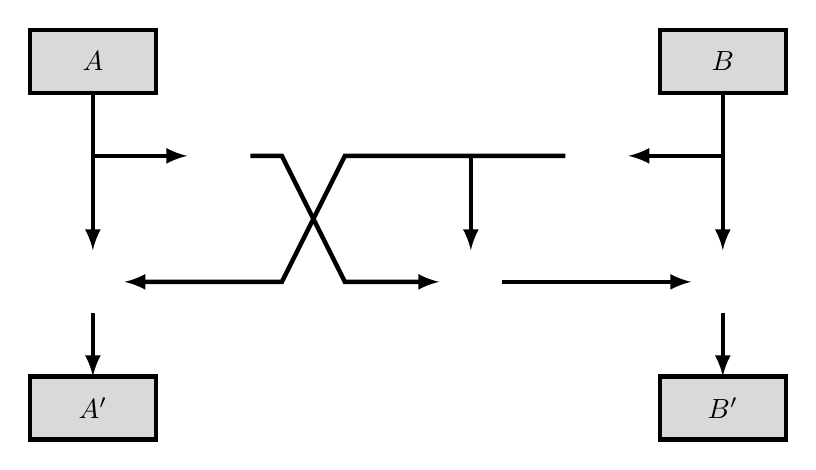
\begin{tikzpicture}[xscale=0.8,yscale=0.8,>=latex,ultra thick]
% Reference grid (temporary)
%\draw[help lines] (0,0) grid (16,16);

% Inputs
\draw[fill=gray!30] (0,15) rectangle (2,14) node[midway] {$A$};
\draw[fill=gray!30] (10,15) rectangle (12,14) node[midway] {$B$};

\draw[->] (1,14) to (1, 11.5);
\draw[->] (1,13) to (2.5, 13);

\draw[->] (11,14) to (11, 11.5);
\draw[->] (11,13) to (9.5, 13); 

\drawxTimes{3}{13}
\drawxTimes{9}{13}

\drawXOR{1}{11}
\drawXOR{11}{11}
\drawXOR{7}{11}

\draw[->] (3.5,13) to (4,13) to (5,11) to (6.5,11);
\draw[->] (8.5,13) to (5,13) to (4,11) to (1.5,11); 
\draw[->] (7,13) to (7,11.5);
\draw[->] (7.5,11) to (10.5,11);

\draw[->] (1,10.5) to (1,9.5);
\draw[->] (11,10.5) to (11,9.5);

% Outputs
\draw[fill=gray!30] (0,9.5) rectangle (2,8.5) node[midway] {$A'$};
\draw[fill=gray!30] (10,9.5) rectangle (12,8.5) node[midway] {$B'$};

\end{tikzpicture}

\caption{Hardware implementation of the forward mixer function.}
\label{fig:MixerMatrix}
\end{figure}

The $x*$ operation is a multiplication by $x$ in \gfsixteen.
Its implementation, which is shown in Figure~\ref{fig:xTimes}, is very simple. 
Notice that a multiplication by $x$ is simply a left rotation followed by a reduction if the MSB was one.
The reduction is derived from the fact that
\begin{equation*}
x^{16} \equiv x^5 + x^3 + x^2 + 1 \bmod{p(x)}
\end{equation*}
for our particular irreducible polynomial $p(x)$, and it is implementable using just three XOR gates.

\begin{figure}[ht]
\centering
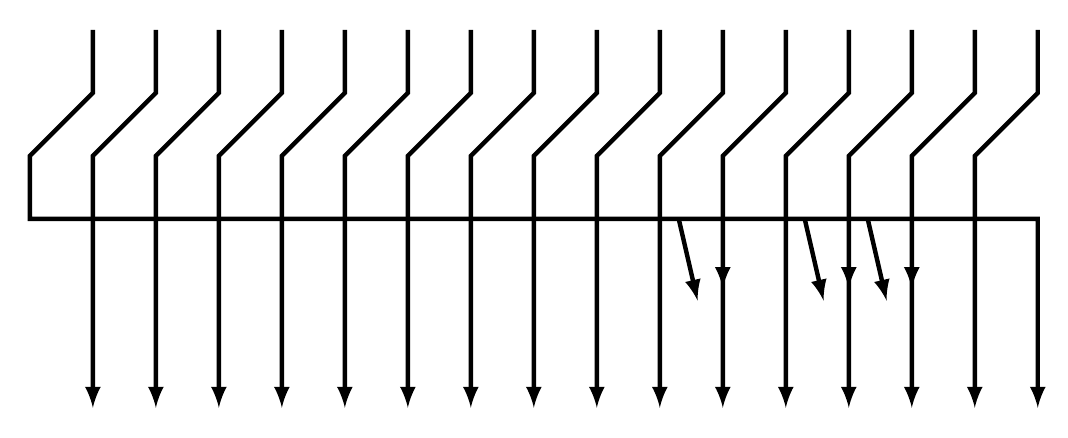
\begin{tikzpicture}[xscale=0.8,yscale=0.8,>=latex,ultra thick]
% Reference grid (temporary)
%\draw[help lines] (0,0) grid (24,24);

\draw[->] (1,24) to (1,23) to (0,22) to (0, 21)
    to (16, 21) to (16, 18);
\foreach \i in {2,...,16} {
    \draw[->] (\i,24) to (\i,23) to (\i-1,22) to (\i-1, 18);
}
\draw[->] (10.3,21) to (10.6,19.7);
\draw[->] (11,21) to (11,19.9);
\drawXOR{11}{19.5}
\draw[->] (12.3,21) to (12.6,19.7);
\draw[->] (13,21) to (13,19.9);
\drawXOR{13}{19.5}
\draw[->] (13.3,21) to (13.6,19.7);
\draw[->] (14,21) to (14,19.9);
\drawXOR{14}{19.5}
\end{tikzpicture}

\caption{Hardware implementation of the $x*$ function. The leftmost bit is the MSB.}
\label{fig:xTimes}
\end{figure}

\subsection{Add Round Constant Step}
The add round constant step is the simplest by far, and it is its own inverse.
A constant $512$-bit value is added to the state using bitwise XOR in order to disrupt symmetry and prevent slide attacks.
The round constant $RC_i$ for round $i$ is given by the formula
\begin{equation*}
RC_i = \mathbf{SHA3\textbf{-}512}(\mathbf{ASCII}(i)),
\end{equation*}
where $\mathbf{ASCII}(i)$ is a function that provides the one or two byte ASCII representation of $i$ and $\mathbf{SHA3\textbf{-}512}$ is the SHA-3 hash function that outputs a $512$-bit message digest. 
Table~\ref{tab:RC} provides the values of $RC_i$ up to $i = 16$.

\makeatletter
\preto{\@verbatim}{\topsep=1em \partopsep=0pt \parskip=0pt \parsep=0pt}
\makeatother

\renewcommand{\arraystretch}{0}

\begin{table}[p]
\begin{tabular}{m{0.1\textwidth}|m{0.8\textwidth}}
\textbf{Constant} & \textbf{Hex Value} \\
& \\

\hline
\centering
$RC_1$ & 
\footnotesize
\begin{verbatim}
00197a4f5f1ff8c356a78f6921b5a6bfbf71df8dbd313fbc5095a55de756bfa1
ea7240695005149294f2a2e419ae251fe2f7dbb67c3bb647c2ac1be05eec7ef9
\end{verbatim}

\\ \hline
\centering
$RC_2$ & 
\footnotesize
\begin{verbatim}
ac3b6998ac9c5e2c7ee8330010a7b0f87ac9dee7ea547d4d8cd00ab7ad1bd5f5
7f80af2ba711a9eb137b4e83b503d24cd7665399a48734d47fff324fb74551e2
\end{verbatim}

\\ \hline
\centering
$RC_3$ & 
\footnotesize
\begin{verbatim}
ce4fd4068e56eb07a6e79d007aed4bc8257e10827c74ee422d82a29b2ce8cb07
9fead81d9df0513bb577f3b6c47843b17c964e7ff8f4198f32027533eaf5bcc1
\end{verbatim}

\\ \hline
\centering
$RC_4$ & 
\footnotesize
\begin{verbatim}
5058cb975975ceff027d1326488912e199b79b916ad90a3fe2fd01508cd7d7c0
1bc8aaa4d21a8473fb15f3b151ab9e44172e9ccb70a5ea04495af3ec03b5153e
\end{verbatim}

\\ \hline
\centering
$RC_5$ & 
\footnotesize
\begin{verbatim}
84da272d13a44f0898ee4ea53334c255d894cc54d357c55466d760debde482a2
44c128df641e80673a8bc34a1620d880b7965e549f313ddccfd506b073413b87
\end{verbatim}

\\ \hline
\centering
$RC_6$ & 
\footnotesize
\begin{verbatim}
bb93aaa23b38ea96c9346ef91e184982bf50e91033f4354ecb20d3c7390c2b41
862e8825ec3d0fee0a6f978881f90728c6748e4aed8b732350075d6c2bdd8e4b
\end{verbatim}

\\ \hline
\centering
$RC_7$ & 
\footnotesize
\begin{verbatim}
fe32f3eba76626dedf36622bfdc5ccd33db2f3e0dd7c3c128298ea78c1cc7fee
1a140edb8e57cd5824c7f4b817c0fc94e70da5b9399faaf9a848a46ad30679e9
\end{verbatim}
  
\\ \hline
\centering
$RC_8$ & 
\footnotesize
\begin{verbatim}
952ba02486b818febc0ec98559df27c79357838f011b1e5bc11f2cfb6fc0573e
545978c2bc5b390f44907f8da0dfd68206fe4521f86ba6c879ec1e69caed9533
\end{verbatim}
  
\\ \hline
\centering
$RC_9$ & 
\footnotesize
\begin{verbatim}
b41e6bb4ed20294016399c268da6bf88c89e2dc118a361b3560ee8daed973a8f
9778df40e308c1206fa42f97f3fd3f63d2b4b3b57eb5bcbec6ad64d46216b692
\end{verbatim}
  
\\ \hline
\centering
$RC_{10}$ & 
\footnotesize
\begin{verbatim}
6954a418cecc43633bd526c2499dfc16b832f58b216b9a8b226a6a0b7918d364
a7939004339de0ba08e2b547e64dc5622e24b0c4f8f415d9e0a84cb94b6c5f3f
\end{verbatim}
  
\\ \hline
\centering
$RC_{11}$ & 
\footnotesize
\begin{verbatim}
2e4b9ad37091e3e5a218c5e57b33ed3470ba4f31fbcf16424684fdd5cde38e88
9eae3f018b37af58c24ccc8af57abc2c6911408dd20ef6435e4494a3e6599a06
\end{verbatim}
  
\\ \hline
\centering
$RC_{12}$ & 
\footnotesize
\begin{verbatim}
aa42aca73bd7f8a17e987f281422b266e44f0de1615d2d393c620c8c5a2c80b4
f06178c8455bf98179603f2f1bcb30b2559f282c799e40533b0665f97a2a706a
\end{verbatim}
  
\\ \hline
\centering
$RC_{13}$ & 
\footnotesize
\begin{verbatim}
969c39ae2dc16834310344c0579d0ffdfde01772dbf9a4cab984953c395d7791
1510f39e5f37295e3611a1d46101460daf731ddbdab1ec1bbc512edc44680d8d
\end{verbatim}
  
\\ \hline
\centering
$RC_{14}$ & 
\footnotesize
\begin{verbatim}
8a1e6ce31f0b526d884b584aa1a5ae4294fcf85fd2e525f959ed1a54233359c7
c5fece6d24775e7d4a9ad97c2632a3be5b331a8f580f557b269e7b65123a5992
\end{verbatim}
  
\\ \hline
\centering
$RC_{15}$ & 
\footnotesize
\begin{verbatim}
9bd64a932f09672def04b6a94753a3e4087a1c3895078dc70927fcd774888dfd
400b95fd1c6a0b2a91a1ba44eea09f5163dba4dfa9da7b8eb97d791cab566437
\end{verbatim}
  
\\ \hline
\centering
$RC_{16}$ & 
\footnotesize
\begin{verbatim}
48401f65c2d2d9e71fe47bd80b28d834eee8fff3be9aa4608cba33e6fedce0b1
693c80cdc36db7f504e4abea23ccc6729a030f5b3e035fb59c2c788215cf84a8
\end{verbatim}

\end{tabular}
\caption{Round constants for up to $16$ rounds}
\label{tab:RC}
\end{table}

\renewcommand{\arraystretch}{1}


\section{Number of Rounds}
This algorithm uses $10$ rounds for a $128$-bit key and $16$ rounds for a $256$-bit key.
The number of rounds is determined, as is typical with block ciphers and permutations, by calculating the number needed for resistance to linear and differential cryptanalysis and adding some buffer to increase the security margin. 
For a more in-depth treatment, refer to Chapter~\ref{ch:Cryptanalysis}.

\section{Customization}
While a specific instantiation is specified here, our algorithm is highly customizable within our security margin.
This could be useful in the case that different users want unique, proprietary algorithms.
We list several possible customizations here.

\subsection{State Initialization}
In the given specification, the inner state (like the outer state) is initialized to zero.
This is not a requirement; indeed, the inner state could be initialized to any $384$-bit value.
Each user could generate their own unique value to set during the initialization phase.
This happens before the first mute calls that absorb the key.

\subsection{S-boxes}
The AES-inspired S-box used here is efficiently implementable in hardware.
There are certainly many other cryptographically secure $16$-bit S-boxes, but randomly generated ones may not be suitable for hardware implementation due to size constraints.
This is an area for further research.
Still, several other AES-like $16$-bit S-boxes are presented in \cite{Wood2013_SboxThesis}.
Any new S-box introduced into the algorithm shall be analyzed to determine its linear and differential characteristics and the number of rounds should be adjusted accordingly if necessary.

\subsection{Bitwise Permutations}
The bitwise permutation provided in the specification is subject to the constraints explained before.
There are many permutations that satisfy these constraints.
We chose to use a permutation that is easily definable by an affine function as obtained by our script; this is not a requirement.
A user could generate their own bitwise permutation subject to the given constraints via exhaustive search.

\subsection{Mixers}
Our mixer is based on a specific $2 \times 2$ matrix multiplication in \gfsixteen modulo a specific irreducible polynomial $p(x)$.
Many matrices are expected to satisfy the constraints that we impose.
These constraints are:
\begin{enumerate}
\item The matrix should be invertible in $\gfsixteen /\left\langle p(x) \right\rangle$
\item The matrix should have differential and linear branch number equal to three (the maximum possible; see Chapter~\ref{ch:Cryptanalysis})
\item The transformation should be efficiently implementable in hardware
\end{enumerate}
Note that the inverse transformation need not be efficiently implementable.
Like the addition of a new S-box, any new mixer (i.e.\ matrix) introduced to the algorithm should be analyzed to ensure it meets these constraints.
A transformation defined by $2 \times 2$ matrix multiplication that does meet the second requirement, for example, would lower our security margin and possibly require increasing the number of rounds significantly.

It should be noted that before settling on a mixer based on matrix multiplication, many mixers based on modular addition, XOR, and rotation operations were tested.
Systems or operations that rely mainly on these operations are typically called \emph{ARX-based}.
None of the ARX-based mixers we tested met our requirement of increasing the branch number from two to three.
However, for completeness, we enumerate all of the mixers examined in this work in Appendix~\ref{appx:ARX_Mixers}.

\subsection{Round Constants}
The round constants presented here are based on SHA-3 hash values.
However, they could be any values that satisfy the following constraints.
Round constants should be:
\begin{enumerate}
\item Unique for each round; to prevent against slide attacks
\item Random, pseudorandom, or highly asymmetric; to reduce symmetry in the state
\end{enumerate}
The round constants are not expected to have any cryptographic significance outside of this.
Different users can generate their own unique set of round constants without difficulty.

There are also other ways of injecting asymmetry into the algorithm using constants.
For example, the round constants could actually be rotation constants that define the amount to rotate each word on the inputs to mixers.

